\begin{frame}
    \begin{center}
        \small
        Волгоградский Государственный Технический Университет \\
        Факультет электроники и вычислительной техники \\
        Кафедра САПРиПК \\
        \vspace{1.5cm}
        \normalsize
        \textbf{Метод построения маршрутов общественного транспорта на основе 
        предпочтений жителей.}\\
        \vspace{1.0cm}
        \raggedleft\small
        \textbf{Исполнитель:}\\Голубев~А.~В.\\
        \textbf{Руководитель:}\\Щербаков~М.~В.\\
        \vspace{1.5cm}
        \vspace{\fill}
        \centeringВолгоград \the\year
    \end{center}
\end{frame}

\begin{frame}
    \frametitle{Формулировка проблемы}
    \textbf{Актуальность.} Изменения в городской среде требуют формирования новых 
    механизмов планирования инфраструктуры города. Для получения эффективных 
    результатов, следует осуществлять принятие решений на основе актуальных 
    данных, отражающих предпочтения жителей.\\
    \textbf{Объект исследования} -- построения маршрутов общественного транспорта.\\
    \textbf{Предмет исследования} -- методы построения маршрутов учитывающие предпочтения жителей.
\end{frame}

\begin{frame}
    \frametitle{Цели и задачи}
    \textbf{Цель работы} -- разработка метода генерации маршрутов общественного 
    транспорта на основе предпочтений жителей для минимизации дискомфорта 
    перемещения в городе. \\
    \textbf{Теоретические задачи:}
    \begin{itemize}\itemsep-5pt
        \item разработка алгоритма обхода кластеров;
        \item построение маршрута по заданным критериям;
        \begin{itemize}\itemsep-5pt
            \item предпочтения жителей;
            \item длина маршрута;
            \item и д.р.
        \end{itemize}
        \item разработка критериев для оценки качества построенного маршрута;
    \end{itemize}
    \textbf{Практические задачи:}
    \begin{itemize}\itemsep-5pt
        \item генерация исходных данных;
        \item реализация разработанных алгоритмов и методов;
        \item построение полученных маршрутов на карте;
        \item оценка качества построенных маршрутов.
    \end{itemize}
\end{frame}

\begin{frame}
    \frametitle{Понятийный аппарат}
    \footnotesize
    \begin{itemize}\itemsep-5pt
        \item \textbf{framework (фреймворк)} -- программная платформа, определяющая структуру 
            программной системы; программное обеспечение, облегчающее разработку и объединение разных 
            компонентов большого программного проекта.
        \item \textbf{OpenStreetMap (OSM)} -- некоммерческий веб-картографический проект по созданию 
            силами сообщества участников-пользователей Интернета подробной свободной и бесплатной 
            географической карты мира.
        \item \textbf{OSRM} -- фреймворк для вычисления кратчайших путей в графе дорог. Разработана 
            для использования с картографическим сервисом OSM.
        \item \textbf{node (точка)} -- точка с указанными координатами;
        \item \textbf{way (линия)} -- упорядоченный список точек, составляющих линию или полигон;
        \item \textbf{relation (отношение)} -- группы точек, линий и других отношений, которым 
            назначаются некоторые свойства;
        \item \textbf{tag (тег)} -- пары <<ключ -- значение>>, могут назначаться точкам, линиям и 
            отношениям.
    \end{itemize}
\end{frame}

\begin{frame}
    \frametitle{Список литературы}
    \begin{enumerate}
        \scriptsize
        \item[1] Bast,~H. Route Planning in Transport Networks [Electronic resource]~/ 
            Hannan Bast at al.~--- Available at:
            \url{http://research.microsoft.com/pubs/207102/MSR-TR-2014-4.pdf}\\
        \item[2] Harabor,~D. Online Graph Pruring for Pathfinding on Grid Maps [Electronic resource]~/ 
            Daniel Harabor and Alban Grastien.~--- Available at:
            \url{http://users.cecs.anu.edu.au/~dharabor/data/papers/harabor-grastien-aaai11.pdf}\\
        \item[3] Geisberger,~R. Contraction Hierarchies: Faster and Simpler Hierarchical Routing in Road 
            Networks [Electronic resource]~/ Robert Geisberger, Peter Sanders, Dominik Schultes, and 
            Daniel Delling.~--- Available at:
            \url{http://algo2.iti.kit.edu/schultes/hwy/contract.pdf}\\
        \item[4] Панченко,~Т.~В Генетические алгоритмы [Текст] : учебно-методическое пособие / под 
            ред.~Ю.~Ю.~Тарасевича. -- Астрахань : Издательский дом <<Астраханский университет>>, 2007. -- 
            87 [3] с.\\
        \item[5] Chu-Hsing,~L. Генетический алгоритм для определения минимального времени пути в 
            интеллектуальных транспортных система [Электронный ресурс] : перевод с английского 
            Казакова~Ю.~С. ~/ Chu-Hsing Lin, Jui-Ling Yu, Jung-Chun Liu, Chia-Jen Lee.~--- 
            Режим доступа:
        \url{http://masters.donntu.org/2010/fknt/kazakovaj/library/translate1.htm}
        \item[6] Басараб,~М.~А. Алгоритмы решения задачи быстрого поиска пути на географических картах / 
            УДК 519.16. -- Москва : МГТУ им. Н.~Э.~Баумана~.--- Режим доступа:
            \url{http://engjournal.ru/articles/1054/1054.pdf}
    \end{enumerate}
\end{frame}

\begin{frame}
    \frametitle{Пассажиропотоки}
    \begin{figure}
        \center
        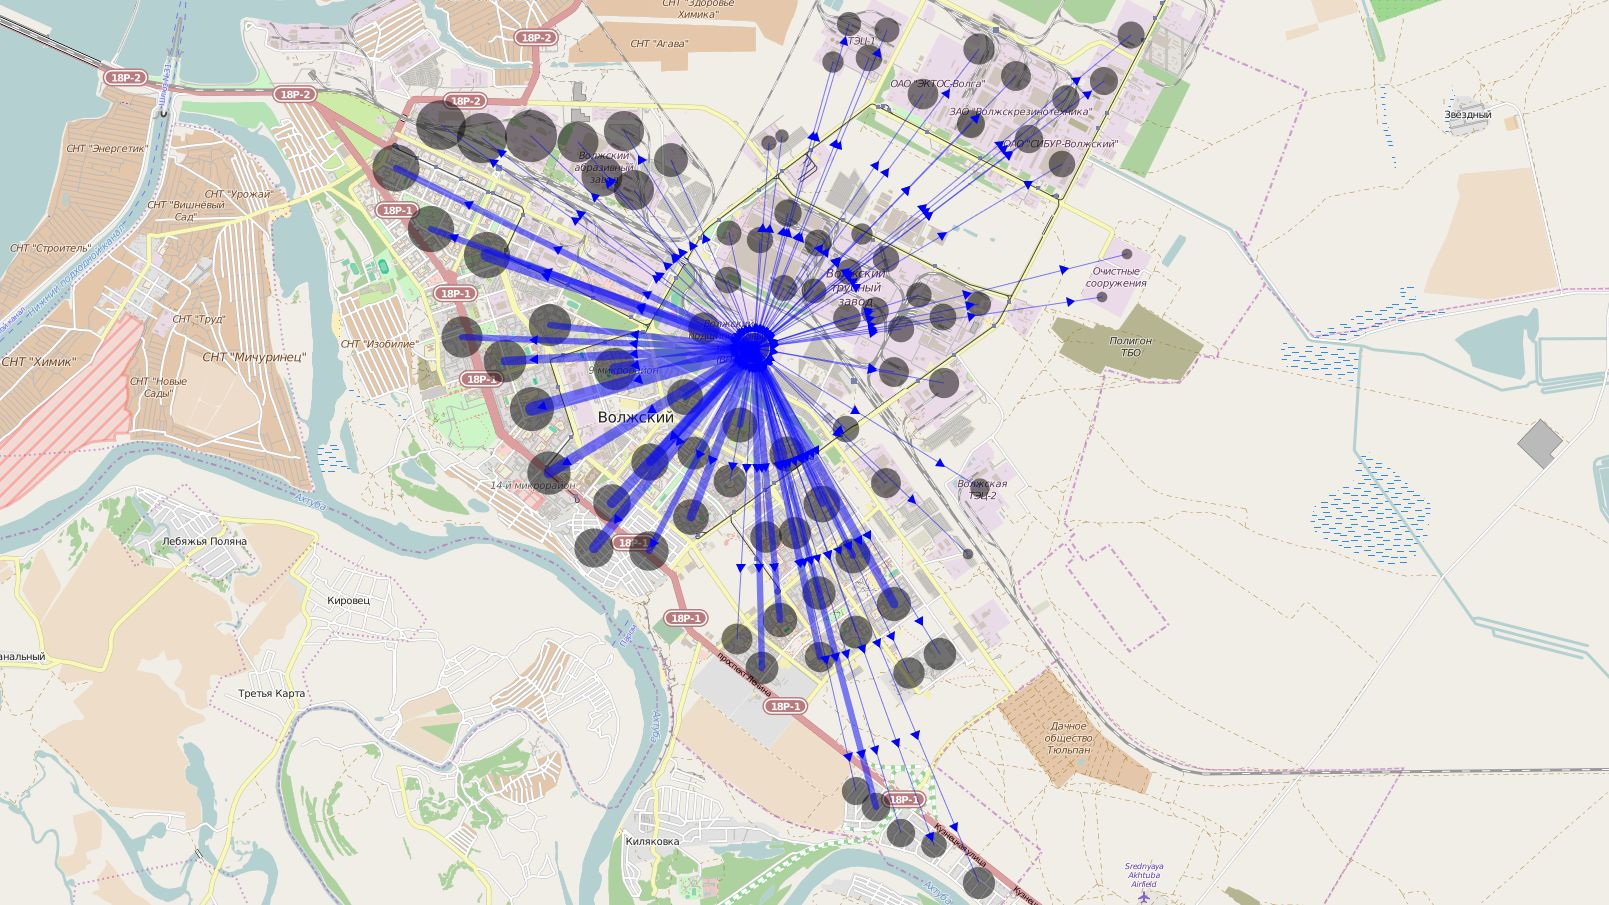
\includegraphics[width=\textwidth]{img00}
    \end{figure}
\end{frame}

\begin{frame}
    \frametitle{Используемый алгоритм}
    Псевдокод алгоритма имитации отжига:\\
    1. \( S \leftarrow \) начальное решение\\
    2. \textbf{repeat}\\
    3. \hspace*{2em} \textbf{выбрать} случайное решение \( R \) из окружение \( S \)\\
    4. \hspace*{2em} \( \Delta \leftarrow f(R) - f(S) \)\\
    5. \hspace*{2em} \textbf{if} \( \Delta < 0 \) \textbf{then} заменить \( S \) на \( R \)\\
    6. \hspace*{2em} \textbf{else} заменить \( S \) на \( R \) c вероятностью \( e^{-\Delta/T} \)\\
    7. \textbf{return} \( S \)
    \footnotetext{где \( T \) -- темпертура процесса, \( f \) -- целевая функция, 
        \( S \) -- исходное решение, \( R \) -- решение кандидат}
\end{frame}

\begin{frame}
    \frametitle{До оптимизации}
    \begin{figure}
        \center
        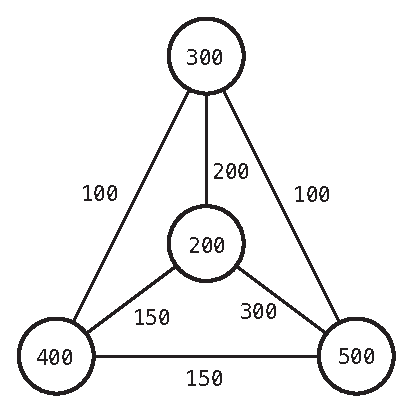
\includegraphics[width=\textwidth]{img01}
    \end{figure}
\end{frame}

\begin{frame}
    \frametitle{После оптимизации}
    \begin{figure}
        \center
        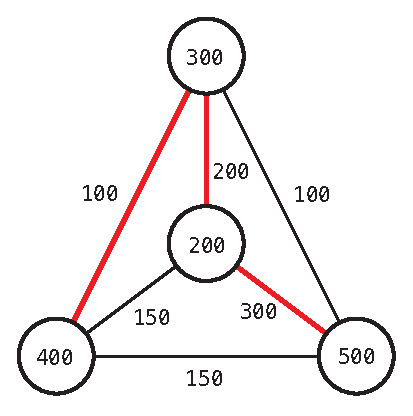
\includegraphics[width=\textwidth]{img02}
    \end{figure}
    \small\emph{Реализованный алгоритм:} \url{https://github.com/vstu-cad-stuff/routing}
\end{frame}

\begin{frame}
    \frametitle{Прототип}
    \begin{figure}
        \center
        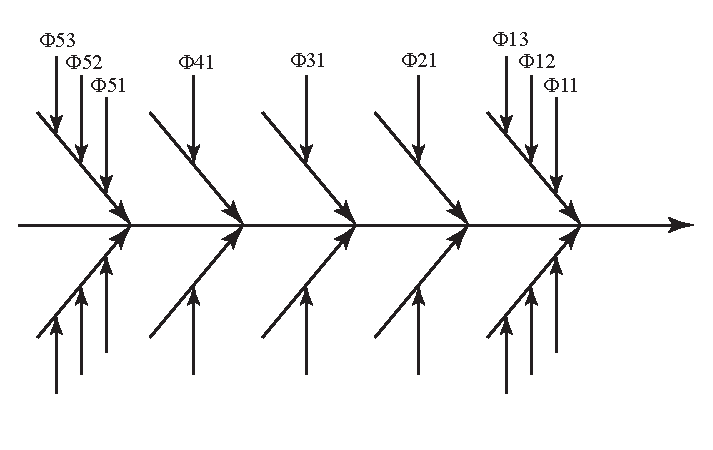
\includegraphics[width=\textwidth]{img03}
    \end{figure}
    \small\emph{Ссылка на приложение:} \url{http://vstu-cad-stuff.github.io/routing/experimental/}
\end{frame}